\documentclass[border=6pt]{standalone}
\usepackage{tikz}
\usetikzlibrary{arrows.meta,positioning,calc,shapes.geometric,fit,backgrounds,patterns,matrix,decorations.pathreplacing}
\begin{document}
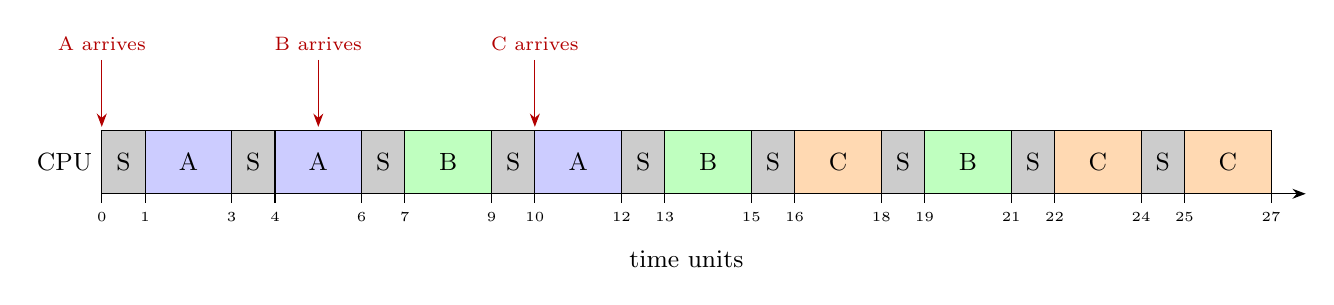
\begin{tikzpicture}[>=Stealth,font=\small]
\def\u{0.55}
\foreach \s/\e/\l/\c in {0/1/S/gray!40,1/3/A/blue!20,3/4/S/gray!40,4/6/A/blue!20,6/7/S/gray!40,7/9/B/green!25,9/10/S/gray!40,10/12/A/blue!20,12/13/S/gray!40,13/15/B/green!25,15/16/S/gray!40,16/18/C/orange!30,18/19/S/gray!40,19/21/B/green!25,21/22/S/gray!40,22/24/C/orange!30,24/25/S/gray!40,25/27/C/orange!30}
 \draw[fill=\c] (\s*\u,0) rectangle node{\l} (\e*\u,0.8);
\node[left] at (0,0.4) {CPU};
\draw[->] (0,0) -- (27.8*\u,0);
\foreach \x in {0,1,3,4,6,7,9,10,12,13,15,16,18,19,21,22,24,25,27}
 \draw (\x*\u,0) -- (\x*\u,-0.12) node[below,font=\tiny]{\x};
\foreach \x/\n in {0/A,5/B,10/C}
 \draw[->,red!70!black] (\x*\u,1.7) node[above,font=\scriptsize]{\n\ arrives} -- (\x*\u,0.85);
\node[below] at (13.5*\u,-0.6) {time units};
\end{tikzpicture}
\end{document}
